\documentclass[12pt]{article}
\usepackage{amsmath}
\usepackage{amsfonts}
\usepackage{amssymb}
\usepackage{subfig}
\usepackage{graphicx}
\usepackage{float}
%\usepackage[cm]{fullpage}

\newcommand{\dbar}{d\mkern-6mu\mathchar'26} 

%%%%% TIKZ CODE (For Feynman diagrams)
\usepackage{tikz}
\usetikzlibrary{arrows,shapes}
\usetikzlibrary{trees}
\usetikzlibrary{matrix,arrows} 				% For commutative diagram
											% http://www.felixl.de/commu.pdf
\usetikzlibrary{positioning}				% For "above of=" commands
\usetikzlibrary{calc,through}				% For coordinates
\usetikzlibrary{decorations.pathreplacing}  % For curly braces
\usetikzlibrary{backgrounds}  				% For showing background grid
\usepackage{pgffor}							% For repeating patterns

\usetikzlibrary{decorations.pathmorphing}	% For Feynman Diagrams
\usetikzlibrary{decorations.markings}
\usetikzlibrary{snakes}
\tikzset{
	% >=stealth', %% Different kind of arrows
    vector/.style={decorate, decoration={snake}, draw},
    fermion/.style={draw=black, postaction={decorate},
        decoration={markings,mark=at position .55 with {\arrow[draw=black]{>}}}},
    fermionbar/.style={draw=black, postaction={decorate},
        decoration={markings,mark=at position .55 with {\arrow[draw=black]{<}}}},
    fermionnoarrow/.style={draw=black},
    gluon/.style={decorate, draw=
        decoration={coil,amplitude=4pt, segment length=5pt}},
    scalar/.style={dashed,draw=black, postaction={decorate},
        decoration={markings,mark=at position .55 with {\arrow[draw=black]{>}}}},
    scalarbar/.style={dashed,draw=black, postaction={decorate},
        decoration={markings,mark=at position .55 with {\arrow[draw=black]{<}}}},
    scalarnoarrow/.style={dashed,draw=black},
%
%% 	Special vectors (when you need to fine-tune wiggles)
	provector/.style={decorate, decoration={snake,amplitude=2.5pt}, draw},
	antivector/.style={decorate, decoration={snake,amplitude=-2.5pt}, draw},
}



\textwidth 6.5in
\oddsidemargin 0in
\evensidemargin 0in
\textheight 8.6in
\topmargin -0.5in
\pagestyle{empty}
\begin{document}

\vspace*{-1cm}
\begin{center}
{\LARGE \bf Relativistic Quantum Field Theory}

\vspace*{0.5cm}
{\Large Physics 7651} \\
\vspace*{0.5cm}
{\Large {\bf Homework 9}\\
\vspace*{0.5cm}
Due: In class on Wednesday, November 2}
\end{center}
\begin{enumerate}



\item {\bf Counter terms on external legs} [5 points]

In class we noted that one does not have to include diagrams with corrections on the external legs. Prove this statement by considering an arbitrary diagram and calculating the overall multiplicative factor associated with summing the series of diagrams formed by including 1PI corrections on a single external leg.

\begin{center}

	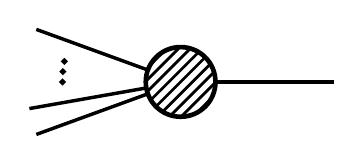
\begin{tikzpicture}[line width=1.25 pt, scale=1.5]
		\draw (200:.3) -- (200:1.3);
		\draw (190:.3) -- (190:1.3);
		\draw (160:.3) -- (160:1.3);
		\draw (0:.3) -- (0:1.3);
%		\draw[fill=black] (185:1) circle (.01);
		\draw[fill=black] (180:1) circle (.01);
		\draw[fill=black] (175:1) circle (.01);
		\draw[fill=black] (170:1) circle (.01);
%		\draw[fill=black] (165:1) circle (.01);
		\draw[fill=black] (0,0) circle (.3cm);
		\draw[fill=white] (0,0) circle (.29cm);
		\begin{scope}
	    	\clip (0,0) circle (.3cm);
	    	\foreach \x in {-.9,-.8,...,.3}
				\draw[line width=1 pt] (\x,-.3) -- (\x+.6,.3);
	  	\end{scope}
	 \end{tikzpicture}
	 \qquad
	 	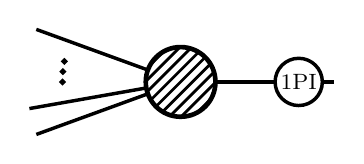
\begin{tikzpicture}[line width=1.25 pt, scale=1.5]
		\draw (200:.3) -- (200:1.3);
		\draw (190:.3) -- (190:1.3);
		\draw (160:.3) -- (160:1.3);
		\draw (0:.3) -- (0:1.3);
%		\draw[fill=black] (185:1) circle (.01);
		\draw[fill=black] (180:1) circle (.01);
		\draw[fill=black] (175:1) circle (.01);
		\draw[fill=black] (170:1) circle (.01);
%		\draw[fill=black] (165:1) circle (.01);
		\draw[fill=black] (0,0) circle (.3cm);
		\draw[fill=white] (0,0) circle (.29cm);
		\begin{scope}
	    	\clip (0,0) circle (.3cm);
	    	\foreach \x in {-.9,-.8,...,.3}
				\draw[line width=1 pt] (\x,-.3) -- (\x+.6,.3);
	  	\end{scope}
	%
		\draw[fill=white] (1,0) circle (.2cm);
		\node at (1,0) {\footnotesize 1PI};
	 \end{tikzpicture}
	 	 \qquad
	 	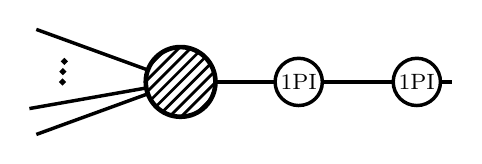
\begin{tikzpicture}[line width=1.25 pt, scale=1.5]
		\draw (200:.3) -- (200:1.3);
		\draw (190:.3) -- (190:1.3);
		\draw (160:.3) -- (160:1.3);
		\draw (0:.3) -- (0:2.3);
%		\draw[fill=black] (185:1) circle (.01);
		\draw[fill=black] (180:1) circle (.01);
		\draw[fill=black] (175:1) circle (.01);
		\draw[fill=black] (170:1) circle (.01);
%		\draw[fill=black] (165:1) circle (.01);
		\draw[fill=black] (0,0) circle (.3cm);
		\draw[fill=white] (0,0) circle (.29cm);
		\begin{scope}
	    	\clip (0,0) circle (.3cm);
	    	\foreach \x in {-.9,-.8,...,.3}
				\draw[line width=1 pt] (\x,-.3) -- (\x+.6,.3);
	  	\end{scope}
	%
		\draw[fill=white] (1,0) circle (.2cm);
		\node at (1,0) {\footnotesize 1PI};
	%
		\draw[fill=white] (2,0) circle (.2cm);
		\node at (2,0) {\footnotesize 1PI};
	 \end{tikzpicture}
\end{center}

\vspace{.5em}

\item {\bf Renormalization of the anharmonic oscillator in QM} [15 points]

Consider an aharmonic oscillator specified by the following Lagrangian,
$$
L = \frac 12 Z \dot{q}^2 - \frac{1}{2} Z_\omega \omega^2 q^2 - Z_\lambda \lambda \omega^3 q^4
$$
We have set $m=1$ so that $\lambda$ is dimensionless.

\begin{enumerate}
\item Find the Hamiltonain $H$ corresponding to $L$ and write it as $H_\text{free} + H_\text{int}$ where $H_\text{free} = \frac 12 P^2 + \frac 12 \omega^2 Q^2$ with $[Q,P]=i$.
%
\item Let $|0\rangle$ and $|1\rangle$ be the ground and first excited states of $H_0$. Let $|\Omega\rangle$ and $| I\rangle$ be the ground and first excited states of $H$. Define $\omega$ to be the excitation energy of $H$, $\omega \equiv E_I - E_\Omega$. We normalize the position operator $Q$ by setting 
$$\langle I |Q |\Omega \rangle = \langle 1 |Q|0\rangle = (2\omega)^{-1/2}. $$
Finally, to make things mathematically simpler, set $Z_\lambda=1$. Write $Z=1+A$ and $Z_\omega=1+B$, where $A=\kappa_A\lambda + \mathcal O(\lambda^2)$ and $B=\kappa_B \lambda +\mathcal O(\lambda^2)$. Use perturbation theory to computer the $\mathcal O(\lambda)$ corrections to the unperturbed energy eigenvalues and eigenstates.
%
\item Find the numerical values of $\kappa_A$ and $\kappa_B$ that yield $\omega=E_I-E_\Omega$ and $\langle I | Q |\Omega \rangle = (2\omega)^{-1/2}$.
%
\item Now think of the Lagrangian above as specifying a quantum field theory in $d=1$ dimensions. Compute the $\mathcal O(\lambda)$ correction to the propagator. Fix $\kappa_A$ and $\kappa_B$ by requiring the propagator to have a pole at $k^2=\omega^2$ with residue one. Do your results agree with those in (c)? Should they?
\end{enumerate}
%
\textit{Hints:} Write $Q$ and $P$ in terms of normalized creation and annihilation operators with $a|n\rangle = \sqrt{n} |n-1\rangle$ and $a^\dag |n\rangle = \sqrt{n+1} |n+1\rangle$. In part (d) use a Wick rotation to calculate the finite loop integral.


\item {\bf Superficial divergences in $\phi^4$} [10 points]

The \textbf{superficial degree of divergence} of a diagram $D$ is the difference in the power of loop momenta in the numerator and the denominator. (This includes the integration measure so that it really gives the naively expected divergence for the expression.)

\begin{enumerate}
\item \textsc{$\phi^4$ theory and EVIL}. (Special Halloween problem.) In $\phi^4$ theory in four dimensions, use power counting to give the expression for the superficial degree of divergence $D$ of a general diagram with $E$ external legs, $V$ vertices, $I$ internal lines, and $L$ loops. Give the relation between $E,V,$ and $I$. Using this and the relation between $L,V,$ and $I$, express $D$ in terms of $E$ and $V$.
\item Given the above result, give a list of all amplitudes which are superficially divergent and give their superficial degree of divergence. Explain why some amplitudes which should be divergent according to (a) are actually not divergent. Specify which counter terms are required. Draw the leading order divergent diagram (including at least one vertex) for each counter term. \textit{Hints: if you can't draw a diagram for an operator, there is usually a reason for this due to symmetry. Make sure that the leading order diagram you draw actually contributes to a given counter term---one counter term is subtle.} 
\item Redo (a) for $\phi^4$ in general spactime dimension $d$. Briefly comment on implications for the superficial degree of divergences in this theory.
\end{enumerate}



%
%
%\item {\bf Don't be afraid of infinities.} [5 points]
%
%\begin{itemize}
%\item Model the `classical' electron as a sphere of charge $e$ and radius $r_e$. Write out the Coulomb self-energy of such an electron, $\Delta E$. This is a contribution to the electron's physical mass,
%$$(m_e^\text{phys})^2 = (m_e^\text{bare})^2 + \Delta E.$$ 
%\end{itemize}
%


%% See also Preskill notes 2.90
%
%\item{\bf The Boltzmann $H$-Theorem} [5 points]
%
%The Boltzmann $H$-theorem is the statement that entropy always increases in an irreversible process. It is often derived in statistical mechanics using the Born approximation or assuming $T$-invariance. Here we will prove it in field theory using unitarity.
%\begin{enumerate}
%
%\item We used $S^\dag S = 1$ to derive the optical theorem. Use $SS^\dag =1$ to prove a very similar relation and hence show that
%$$
%\sum_f \Gamma (a \to f) =  \sum_f \Gamma (f \to a).
%$$
%\item Let $P_i$ be the probability of finding the system in a state $i$. The rate of decrease in $P_i$ due to transitions to other states is $P_i \sum_f \Gamma(i\to f)$ while the rate of increase of $P_i$ due to transitions from all other states is $\sum_f P_f \Gamma(f\to i)$. Show that $\sum_i P_i$ is time-independent. 
%
%\item Entropy is defined as $S = -\sum_i P_i \ln P_i$. Write out the rate of change of entropy. By judicious relabeling of variables, show that this may be written as
%$$
%\frac{dS}{dt} = \sum_{i,f} P_f \ln\left(\frac{P_f}{P_i}\right) \Gamma(f\to i).
%$$
%
%\item Use the inequality
%$$
%y\ln\frac yx \geq y-x
%$$
%and the result of (a) to show that $dS/dt \geq 0$.
%
%
%\end{enumerate}


%11, 18, 2


\end{enumerate}
 

\end{document}
